\chapter{Improved Windowed Coding}
\label{chap-3}
\graphicspath{{Chapter_3/Vector/}{Chapter_3/}}

In this chapter, we discuss the modifications made to the windowed scheme introduced in chapter \ref{chap-2} to improve upon the shortcomings in section \ref{problems}. In the proceeding sections we take up each issue and describe the modifications and their effects. In some cases, since the work is in progress, we describe our thought process and preliminary results.

\section{Experimental Setup}
\rhead{Experimental Setup}
As an initial step, we describe our experimental setup. The windowed coding scheme was simulated in both Python and MATLAB. We are only working on the windowed coding scheme of the paper \cite{borkotokyicc} and will later evaluate the \textit{selective coding} scheme. The feedback implementation was modified to augment the information content along with the improvements to the degree selection already made. A notable difference as stated by the authors of \cite{borkotokyicc} is that there exists a buffer at the receiver in their implementation which stores some recent coded symbols even if no information symbol can be decoded from them. This helps in decoding symbols later when some extra information symbols have been received. Currently, our implementation does not have a buffer at the receiver. But, in our experiments we find the role of the buffer to be minimal but further evaluation needs to be done. One initial roadblock which we faced was similar code in Python and MATLAB diverged on their results. Though, later we decided to stick to MATLAB which provided better results.

\section{Improvements}
\rhead{Improvements}
In this section we describe the modifications made to solve some of the issues in section \ref{problems}. We first describe improved degree selection process followed by improved feedback structure and no feedback degree selection.

\subsection{Improved Coding Degree Selection}
As stated in section \ref{degree-selection} the process of choosing a suitable coding degree is computationally very demanding and the energy and space requirements are too high to be met by any small sensor node. Additionally, the time consumed in calculating the degree is also very high which may prove to be disastrous in high speed applications. 

The optimal degree is chosen by:

\begin{equation} \label{eq:1}
	f(x,y) = \argmax_{d} \left(y\frac{\binom{x-y}{d-1}}{\binom{x}{d}}\right)
\end{equation}

where $x=i-u-1$, $y=\beta-1$ and $f$ is the optimal degree. 

Now, we need to find the maxima of the $f(x,y)$ function which can give us the optimum degree. So instead of searching over the entire domain space of $d$ we use calculus to find the maxima. This optimization though a little involved but the final results are very simple and worth it. We can expand the function $f(x,y)$ as

{\large\[
f(x,y) = \argmax_{d} \left(y\frac{\frac{(x-y)(x-y-1)...(x-y-d+2)}{(d-1)(d-2)...1}}{\frac{x(x-1)(x-2)...(x-d+1)}{d(d-1)...1}}\right)
\]}


\[
f(x,y) = \argmax_{d} 	\left(d*y\frac{(x-y)(x-y-1)...(x-y-d+2)}{x(x-1)(x-2)...(x-d+1)}\right)
\]
\linebreak
Let us assume we need to maximize $g(x,y)$ with

\begin{equation} \label{eq:2}
	g(d) = d*y\frac{(x-y)(x-y-1)...(x-y-d+2)}{x(x-1)(x-2)...(x-d+1)}
\end{equation}
This is only a function of $d$ because $x$ and $y$ are constant at a given time. Take log of this for finding the derivative. In that case:

\begin{equation} \label{eq:3}
	h(d) = \ln d + \ln y + \sum_{k=0}^{d-2}{\ln(x-y-k)} - \sum_{k=0}^{d-1}{\ln(x-k)}
\end{equation}
\linebreak
where $h(d) = \ln(g(d))$. We know the values of x, y and d are integers. So the above function $ln(g(d))$ is discrete and the derivative cannot be calculated in a continuous fashion. We know derivative in discrete domain is

\begin{equation} \label{eq:4}
	y[n] = x[n] - x[n-1]
\end{equation}

Use \ref{eq:4} to find derivate of \ref{eq:3}. This will give the derivate as $h'(d)$ as:

\begin{equation} \label{eq:5}
	h'(d) = \ln({\frac{d}{d-1}}) + \ln(x-y-d+2) - \ln(x-d+1) 	
\end{equation}
For calculating the maxima we need to find the value of $d$ where $h'(d)$ is zero.

\[
\ln({\frac{d}{d-1}}) + \ln(x-y-d+2) - \ln(x-d+1) = 0	
\]

\[
\frac{d}{d-1}. \frac{(x-y-d+2)}{(x-d+1)} = 1	
\]

\[
dx - dy - d^2 + 2d = dx - d^2 -x + 2d - 1
\]

\[
-dy = -x - 1
\]

\begin{equation} \label{eq:6}
	d = \frac{x+1}{y}
\end{equation}

Hence, the optimal degree
\begin{equation} \label{eq:7}
	d = \frac{i-u}{\beta - 1}
\end{equation}
where,
$i$ is the current sequence number, $u$ is the oldest undelivered packet and $\beta$ is the number of undelivered packets. One more caveat of implementation is that the maximum value of degree cannot be greater than the window size - number of undelivered and degree should be integer. To incorporate both the conditions we transform \ref{eq:7} as:

\begin{equation} \label{eq:8}
	d = \min (i-u-\beta, \floor{\frac{i-u}{\beta - 1}})
\end{equation}

It is clear now that Eq \ref{eq:8} provides a better way to calculate the degree. It removes all the complex calculations and now both the space and time complexity of calculating the degree once is $O(1)$. Fig. \ref{opt-degree-fig} shows the result of the simulation when we compare the original degree selection method (Eq. \ref{main-eq}) with our optimized degree selection (Eq. \ref{eq:8}). Both the approaches give similar results as there is no theoretical difference between the two but our optimized approach is computationally very efficient.

\begin{figure}[t]
	\centering
	\includegraphics[width=15cm,height=10cm,keepaspectratio]{my_opt}
	\caption{The results obtained when simulating the original windowed coding scheme (red) and the same coding scheme with better degree optimization (blue). It is clearly visible that the curves are very similar.}
	\label{opt-degree-fig}
\end{figure}


\subsection{Improvised Feedback}
In an earlier section \ref{feedback-issue}, we stated that the feedback is not fully utilized. Even if we $32$ bit feedback we could only know the state of one symbol with certainty. Suppose, we know which other symbols are missing we could directly send them in the next transmission. Each symbol whose state we know will alleviate the need of coding for it. This will greatly reduce the energy consumption at both the receiver's and transmitter's end, which is one of the key requirements of our use case.

We keep the basic structure of the feedback packet (see Fig. \ref{feedback}) intact. In our approach, we only modify the ``number of unexpired undelivered symbols'' section of the feedback, because it is section which is not fully utilized. We use the $15$ bits for a $32$ bit feedback, assigned to that section to pass on information about the other symbols back to the sender. The first $16$ bit section of the feedback provides the sequence number of the oldest undelivered unexpired symbol, $u$,  then we use the next $15$ bit segment to denote whether symbols $s_{u+1}, s_{u+2},...., s_{u+15}$ have been received or not. If any of that symbol is missing that bit would be set. This can help us know about the exact state of the symbols from $[s_u, s_{u+15}]$ so depending on the packet size $b$ we can send the missing symbols directly without coding. The major advantage of this approach is that if the delay tolerance $\delta_{max}$ is less or equal to $16$ we do not need to code for any symbol in the payload $\mathbf{p}_i$, if we have received feedback for the packet $\mathbf{p}_{i-1}$. Coding still needs to be done if we don't receive feedback for the previous packet. This scheme can still work for higher $\delta_{max}$ if we assign more bits to the feedback.

In our use case, the feedback bits also cannot increase arbitrary and they have to follow a limit to respect the duty cycle and energy constraints. So what can be done if $\delta_{max}$ is greater than the feedback bits assigned to state of other symbols? We propose an adaptive scheme in that case. Let us assume the number of bits assigned to the improvised feedback section be $l_b$. Now the set of relevant symbols at time instant $i$, $[s_{u}, s_i]$ can be broken into two disjoint sets $[s_{u}, s_{u+l_b}]$ and $[s_{u+l_b+1}, s_{i}]$ if $i-u > l_b$. The receiver knows the number of missing symbols in both of the sets. The first set contains older packets and they should be transmitted first to ensure that they don't expire. To do that we can use the improvised feedback as the state of all symbols in the first set can be incorporated into the feedback $l_b$ bits. This works if majority of missing symbols are in the first set, but if the majority of symbols are missing in the second set we cannot send information about that set through our improvised method because then the older symbols would stand the risk to expire before delivery. So in this case we would shift back to the original \textit{windowed coding} scheme transmitting the feedback as in Fig. \ref{feedback}. We can control the level of adaptability by defining a constant $\alpha$ as
\begin{equation}
	\alpha = \frac{number\ of\ missing\ symbols\ in\ set\ [s_{u+l_b+1}, s_i]}{number\ of\ missing\ symbols\ in\ set\ [s_{u}, s_{u+l_b}]}
\end{equation}

We can then set a threshold $\alpha_0$. If $\alpha > \alpha_0$ we switch to the original \textit{windowed coding} scheme's feedback structure, else we use the improvised feedback structure to pass information about symbols in the set $[s_{u}, s_{u+l_b}]$. The results of our experiments after making these modifications are shown in the next set of figures.

	
\begin{figure}
	\centering
	\includegraphics[width=15cm,height=10cm,keepaspectratio]{results-delay=4-feed=4-switch}
	\caption{Comparison between baseline Repetition Redundancy (purple), Windowed Coding (yellow), Adaptive scheme (blue) and No coding or improved feedback (red). The simulation is done when delay tolerance $\delta_{max}=4\ and\ l_b=4$. The switching to the original scheme in adaptive takes place instantaneously i.e. $\alpha_0 = 0$. It can be clearly seen that the no coding scheme performs better than everything and it does not employ any coding so is energy efficient too.}
	\label{results-feed-1}
\end{figure}

\begin{figure}
	\centering
	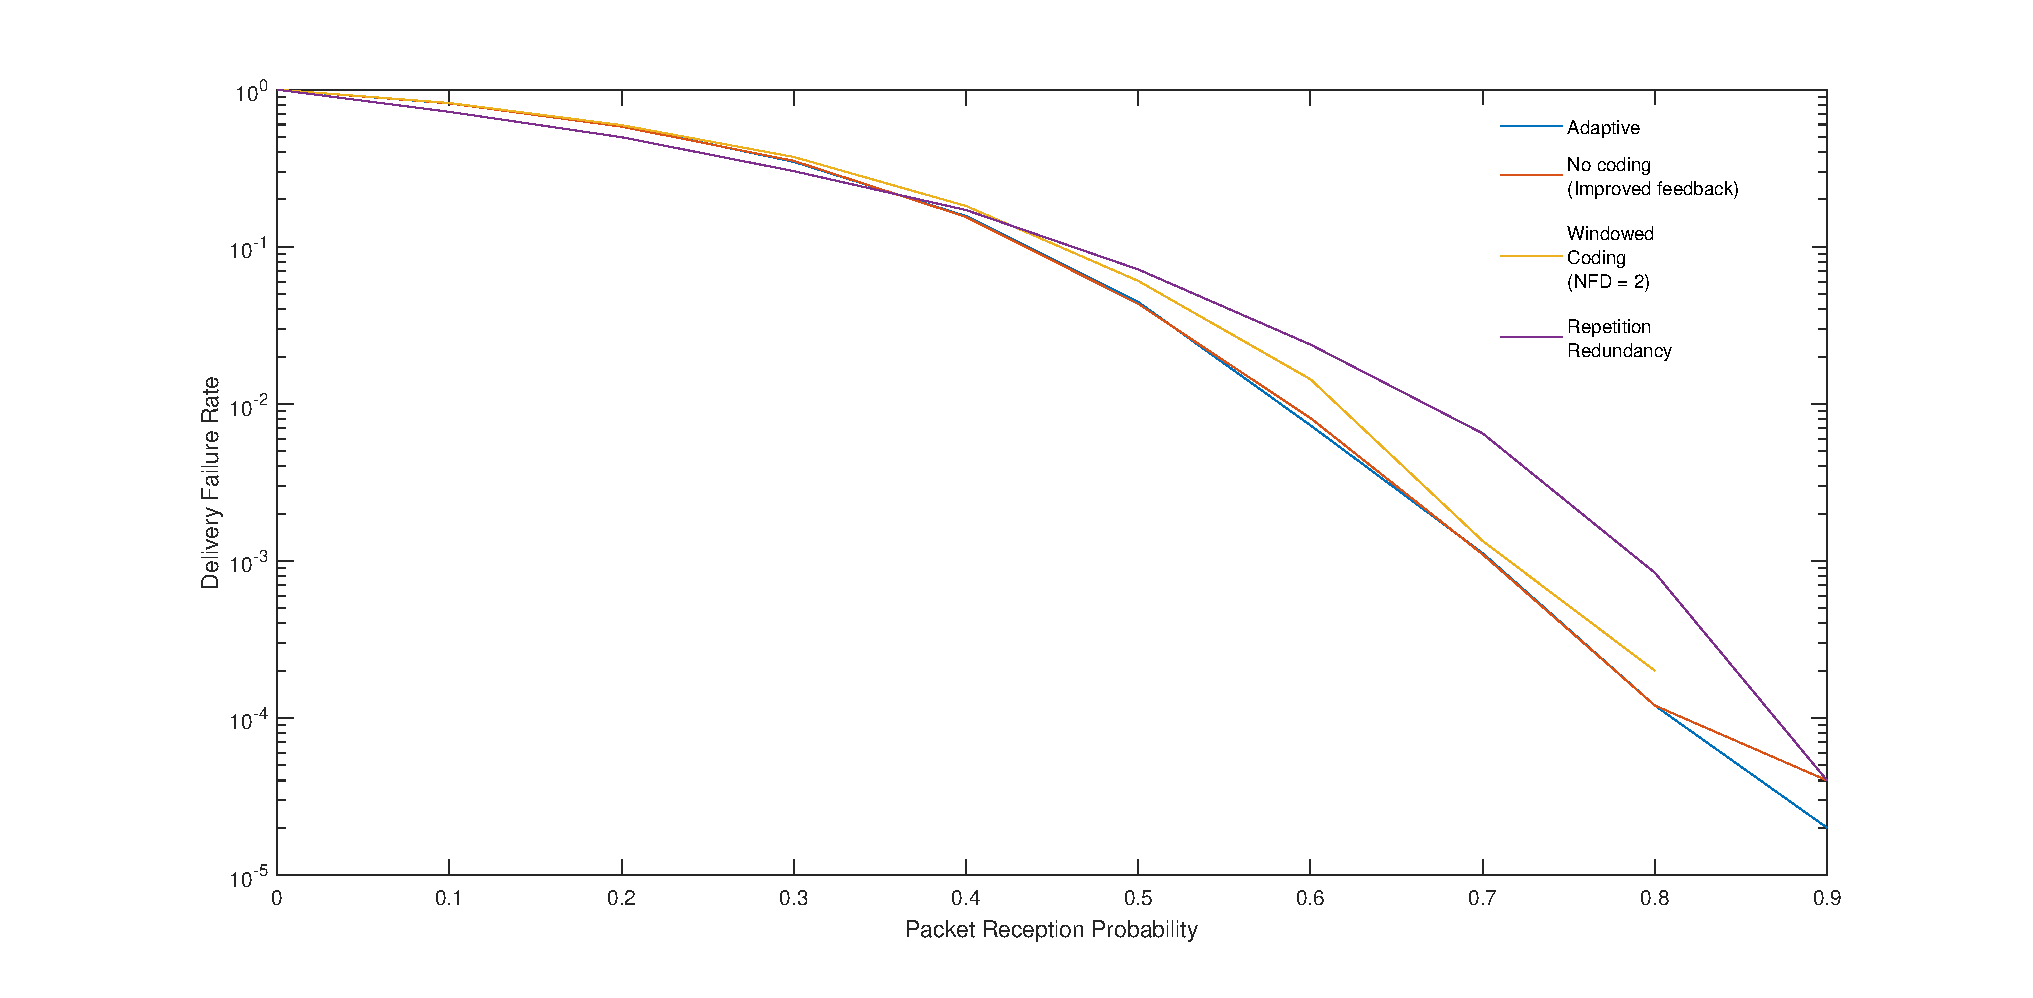
\includegraphics[width=15cm,height=10cm,keepaspectratio]{results-delay=16-feed=4-switch}
	\caption{Similar simulation as in Fig. \ref{results-feed-1} but with $\delta_{max}=16$ i.e $\delta_{max} > l_b$. The no coding performance deteriorates because now most of the missing symbols are outside the range in which it can provide information i.e. in set $[s_{u+l_b+1}, s_i]$.}
	\label{results-feed-2}
\end{figure}

\begin{figure}[t]
	\centering
	\includegraphics[width=15cm,height=10cm,keepaspectratio]{results-delay=16-feed=4-alp=1.5}
	\caption{Similar simulation as in Fig. \ref{results-feed-2} but with $\alpha_0 = 1.5$. The no coding performance is similar to what was before because now also most of the missing symbols are outside the range in which it can provide information i.e. in set $[s_{u+l_b+1}, s_i]$. The adaptive scheme's performance becomes very similar to \textit{windowed coding} because of the transmission take place in the windowed coding mode rather than the improvised feedback mode.\\}
	\label{results-feed-3}
\end{figure}


\subsection{No feedback degree selection}

According to the algorithm of \textit{windowed coding} if feedback for payload $\mathbf{p}_{i-1}$ is not received, then the current payload $\mathbf{p}_{i}$ will contain all coded symbols. The degree of coding is chosen randomly from a uniform distribution between $[1, z]$ where $z = min(i-u_l, i-u_{max})$, $u_l$ is the oldest undelivered sequence in the most recent feedback and $u_{max} = i-\delta_{max}$, the oldest unexpired information symbol at the current instant, $i$. The idea behind this that since no information about the state of symbols is known an assumption is made that all the symbols are equally likely to be missing so a uniform random variable is used to choose the coding degree. But on further thought it is clear that not all symbols have the same probability of missing. The symbols which are older have got more chances in the past to be delivered than recent symbols. In a way the probability of missing should increase for a more recent symbol, but this assumption is only valid if channel erasure is uniform. For Gilbert-Elliot channel where burst errors occur it may be possible that any set of symbols may be lost in a burst and thus no conclusion can be drawn about the missing probability of symbols.

We conduct some experiments with various fixed degrees while coding when no feedback is present. The \textit{Delivery Failure Rate} is quite erratic and sometimes performs even worse than Repetition Redundancy. The best performance is seen when the no feedback coding degree is $2$. There is no clear theoretical understanding why this happens and what should be the optimal no feedback degree for different scenarios. On initial thought, the best performance of $NFD = 2$ can be explained by the decoding process. We know that for successful decoding $d-1$ out of the $d$ combined symbols must already be received. So when the degree is $2$ if anyone among the two is already present decoding is successful but for degree $3$ we would any two of them to be already received and so on for higher degrees. It becomes improbable that atleast $n-1$ symbols are already received for $n$-degree coded symbol as $n$ increases. So most of the transmissions with higher coding degree would not result into a successful deocde and thus the delivery failure rate is higher. 


\begin{figure}[t]
	\centering
	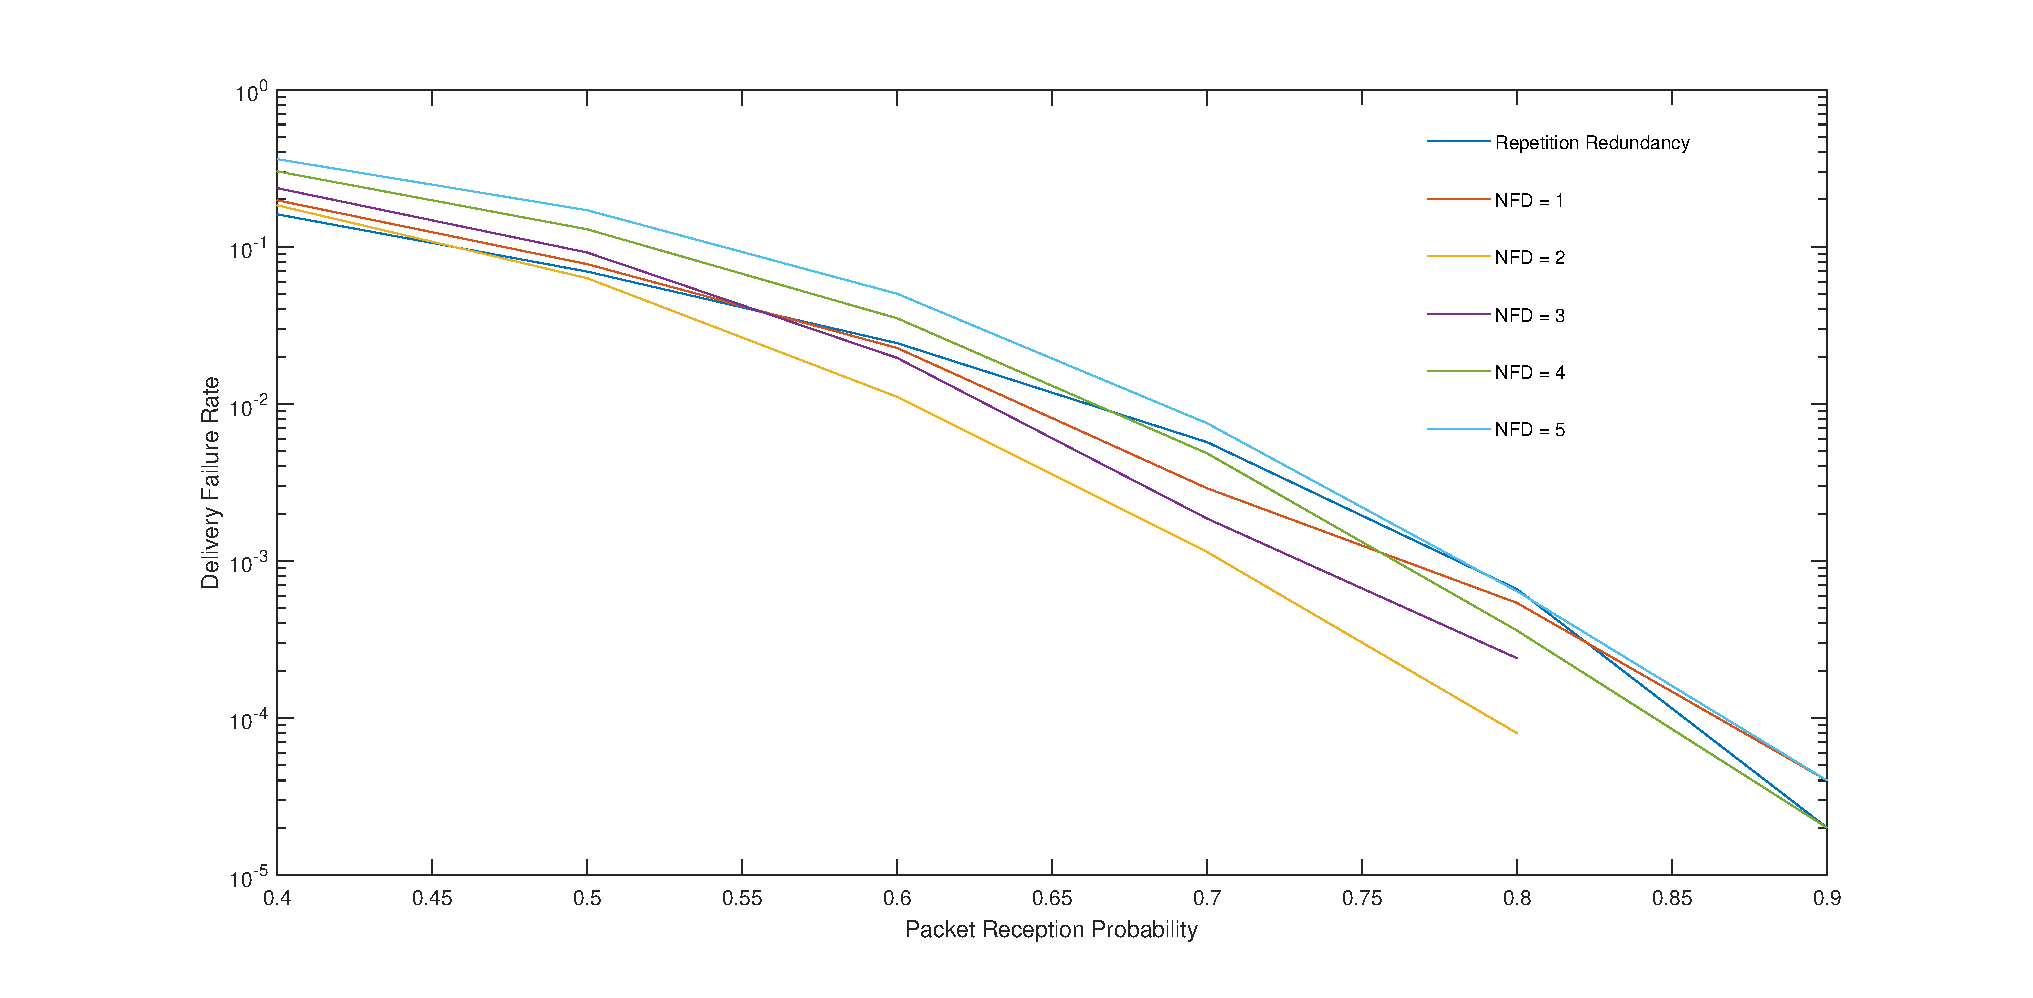
\includegraphics[width=15cm,height=10cm,keepaspectratio]{basic}
	\caption{Delivery Failure Rate v/s Packet Reception Probability with different values of No Feedback Degree (NFD).}
	\label{basic}
\end{figure}


\section{Future Works}
\rhead{Future Works}
In the previous section we have described the analysis that has been completed yet. There are many other things to explore. In coming months our focus will be on the adaptive scheme and how it can be further improved. At the moment, there are some issues with the scheme. Furthermore, there is no theoretical ground to degree selection when there is no feedback. We would explore how to quantify the no feedback state and how to choose optimal degree based on the information which we might have from previous feedback. Even when feedback is present the estimate for optimal degree is suboptimal because when a single payload contains more than one coded symbol joint optimization of degree over both the symbols should be looked into. In this work, the focus has been on the \textit{windowed coding} scheme whereas the paper \cite{borkotokyicc} lists one more algorithm---\textit{selective coding}. \textit{Selective coding} should also be looked into to improve its performance. Apart from all this we also need to evaluate our methods on different channel erasure models as currently we are focusing on Bernouli and Gilbert-Elliot channels. Finally, the role of a buffer at the receiver should also be investigated.


